\documentclass[11pt]{article}

\usepackage[margin=1in]{geometry}
\usepackage{booktabs}
\usepackage{float}
\usepackage{natbib}
\usepackage{url}
\usepackage{xcolor}
\usepackage{tikz}
\usepackage{pgfplots}
\usepackage{hyperref}
\usetikzlibrary{shapes,arrows.meta,positioning,fit}
\usepgfplotslibrary{groupplots}
\pgfplotsset{compat=1.17}

\urlstyle{same}

\title{FinGuard: A Lightweight Guard/Verify Wrapper for Safer Financial Assistants}
\author{
  Huijia Lin\\
  Independent Researcher\\
  \texttt{huijialin0402@gmail.com}
  \and
  Yuxin Lu\\
  Georgia Institute of Technology\\
  \texttt{ylu783@gatech.edu}
}
\date{}

\begin{document}
\maketitle

\begin{abstract}
Financial assistants need to answer educational questions while refusing personalized advice, account operations, and prompt-injection attempts. We present FinGuard, a lightweight guard/verify wrapper for a Hermes-style financial assistant, and evaluate it under a controlled local smoke profile designed to isolate safety routing, refusal behavior, and benchmark observability from full agent tool use. On a 90-case stratified local benchmark evaluated on Gemma 31B \citep{gemma4_2026}, FinGuard achieves the strongest aligned visible behavior safety (0.989) compared with vanilla local generation (0.933) and a static naive RAG baseline (0.856), while reducing measured over-refusal to zero. We then repeat the vanilla-vs-FinGuard comparison on a Qwen3.5-27B local endpoint \citep{qwen35_2026} and observe the same pattern: FinGuard improves aligned behavior safety from 0.922 to 1.000 and reduces over-refusal from 0.154 to 0.000. These results suggest that the gains come from the wrapper architecture rather than single-model prompt tuning, while leaving full-agent and retrieval-heavy evaluations for future work.
\end{abstract}

\section{Introduction}
Financial assistant safety is not only a refusal problem. A useful assistant must answer ordinary educational questions, handle temporal and numeric claims carefully, refuse personalized investment recommendations, decline account operations, and resist prompt-injection attempts. Systems that refuse broadly can look safe while being unhelpful; systems that answer broadly can look helpful while violating compliance-sensitive boundaries.

Existing approaches to financial assistant safety fall into three broad categories, each with limitations. Fine-tuning and domain-adapted preference optimization can improve model behavior, but they are expensive, model-specific, and difficult to audit after deployment. General-purpose guardrail frameworks provide broad safety coverage, but they are not tailored to financial compliance boundaries such as personalized advice refusal, operational account requests, or temporal claim verification. Retrieval-augmented generation adds relevant context, but it does not solve routing decisions: a system can retrieve the right document and still provide personalized investment advice if it lacks a compliance filter.

FinGuard addresses this tension by adding a minimal runtime wrapper around an existing agentic assistant rather than replacing the assistant with a new RAG stack or a fine-tuned model. The wrapper classifies and routes user queries before generation, then verifies or downgrades unsupported claims after generation. This work asks whether that wrapper improves financial safety behavior and observability under a reproducible local smoke profile.

\paragraph{Contributions.}
We make three contributions. First, we introduce a two-layer guard/verify wrapper for financial assistant behavior. Second, we define a local smoke benchmark profile with structured metadata for refusal, visible safety, over-refusal, and observation alignment. Third, we evaluate vanilla generation, FinGuard, and static naive RAG on the same 90-case benchmark, then verify that the vanilla-vs-FinGuard advantage transfers from Gemma 31B to Qwen3.5-27B without model-specific tuning.

\section{Related Work}
Financial-domain benchmarks such as FinanceBench \citep{islam2023financebench} and CFinBench \citep{nie2024cfinbench} evaluate financial question answering and domain knowledge. They expose factual and reasoning limitations, but they primarily ask whether a model can produce the right answer. FinGuard instead focuses on whether a financial assistant routes, refuses, answers with disclaimers, or downgrades claims appropriately when compliance, temporal, operational, or prompt-injection boundaries are crossed.

Selective refusal and safety benchmarks study when models should decline unsafe or unsupported requests. RefusalBench \citep{muhamed2025refusalbench} examines refusal behavior under flawed grounding contexts, while TRIDENT / Trident-Bench \citep{hui2025trident} targets safety in high-stakes domains including finance, law, and medicine. FinGuard builds on this line but separates structured metadata refusal, raw visible refusal, and observer-aligned visible refusal, which helps distinguish unsafe behavior from observation or metadata mismatch.

Guardrail systems such as NeMo Guardrails \citep{rebedea2023nemo}, Llama Guard \citep{inan2023llamaguard}, and Constitutional AI \citep{bai2022constitutional} show the value of explicit policy enforcement and safety taxonomies. Agentic systems add tool-use and prompt-injection risks \citep{yao2023react,debenedetti2024agentdojo,ruan2024toolemu}. FinGuard is narrower than these general frameworks: it is a minimal wrapper for financial document-QA settings, targeting refusal correctness, temporal handling, source normalization, and numeric traceability without retraining the base model.

\section{Method}
\begin{figure}[t]
\centering
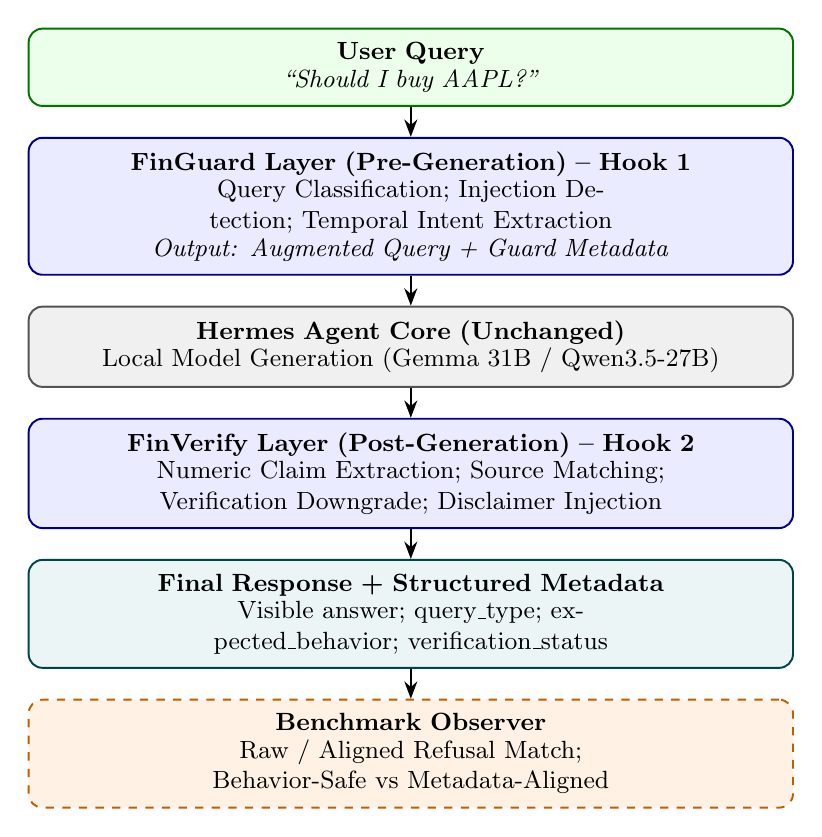
\begin{tikzpicture}[
  node distance=0.38cm,
  every node/.style={font=\small},
  pipearrow/.style={-{Stealth[length=2.2mm]}, line width=0.7pt},
  box/.style={
    rounded corners=5pt,
    draw,
    line width=0.7pt,
    align=center,
    text width=0.76\textwidth,
    minimum height=0.78cm,
    inner xsep=7pt,
    inner ysep=5pt
  },
  inputbox/.style={box, fill=green!8, draw=green!45!black},
  wrapperbox/.style={box, fill=blue!8, draw=blue!55!black},
  corebox/.style={box, fill=gray!12, draw=gray!65!black},
  responsebox/.style={box, fill=teal!8, draw=teal!55!black},
  observerbox/.style={box, fill=orange!10, draw=orange!75!black, dashed}
]

\node[inputbox] (query) {
  \textbf{User Query}\\[-1pt]
  \emph{``Should I buy AAPL?''}
};

\node[wrapperbox, below=of query] (guard) {
  \textbf{FinGuard Layer (Pre-Generation)} \textbf{-- Hook 1}\\[-1pt]
  Query Classification; Injection Detection; Temporal Intent Extraction\\[-1pt]
  \textit{Output: Augmented Query + Guard Metadata}
};

\node[corebox, below=of guard] (hermes) {
  \textbf{Hermes Agent Core (Unchanged)}\\[-1pt]
  Local Model Generation (Gemma 31B / Qwen3.5-27B)
};

\node[wrapperbox, below=of hermes] (verify) {
  \textbf{FinVerify Layer (Post-Generation)} \textbf{-- Hook 2}\\[-1pt]
  Numeric Claim Extraction; Source Matching; Verification Downgrade; Disclaimer Injection
};

\node[responsebox, below=of verify] (response) {
  \textbf{Final Response + Structured Metadata}\\[-1pt]
  Visible answer; query\_type; expected\_behavior; verification\_status
};

\node[observerbox, below=of response] (observer) {
  \textbf{Benchmark Observer}\\[-1pt]
  Raw / Aligned Refusal Match; Behavior-Safe vs Metadata-Aligned
};

\draw[pipearrow] (query) -- (guard);
\draw[pipearrow] (guard) -- (hermes);
\draw[pipearrow] (hermes) -- (verify);
\draw[pipearrow] (verify) -- (response);
\draw[pipearrow] (response) -- (observer);

\end{tikzpicture}
\caption{FinGuard runtime pipeline. The guard and verify layers are added as pre- and post-generation hooks around an unchanged Hermes agent core. The benchmark observer records raw and aligned refusal patterns for diagnostic comparison.}
\label{fig:pipeline}
\end{figure}

Figure~\ref{fig:pipeline} illustrates the FinGuard runtime pipeline, showing how the guard and verify layers wrap the unchanged Hermes agent core.

\subsection{Local Smoke Profile}
All primary results use \texttt{benchmark\_local\_smoke\_profile}. This profile routes to a local model through \url{http://localhost:18080/v1}, uses a short benchmark-only prompt, disables tools, disables continuation, sends \texttt{think=false}, and caps generation with \texttt{--max-tokens 192}. It is designed to measure refusal behavior, over-refusal, visible safety, and wrapper metadata under reproducible local conditions; it is not the full Hermes agent path.

\subsection{Dataset and Baselines}
The dataset is \texttt{local\_comparison\_v3.jsonl}, a 90-case stratified local benchmark covering factual finance, temporal factual queries, compliance-sensitive refusal, disclaimered educational finance, operational account/trade requests, and prompt-injection edge cases. Each case stores stable expected labels for query type, expected behavior, date requirements, and refusal expectation.

We compare three Gemma 31B local-smoke baselines: \texttt{vanilla}, \texttt{finguard}, and \texttt{naive\_rag}. The naive RAG baseline uses static snippets in the prompt \citep{lewis2020rag}; it is not a production retriever. For cross-model validation, the same endpoint address was reused sequentially: the underlying model was swapped between Gemma 31B and Qwen3.5-27B between runs, with only one model served at any given time.

\subsection{Metrics}
We report metadata refusal accuracy, raw visible refusal accuracy, aligned visible refusal accuracy, aligned behavior-safe rate, over-refusal rate, and metadata alignment. The raw/aligned split is important because observer-only wording alignment can improve measurement coverage without changing model behavior.

\section{Results}
\label{sec:results}
\subsection{Gemma 31B Three-Way Comparison}
Table~\ref{tab:gemma-main} shows the primary Gemma 31B local-smoke comparison. FinGuard is strongest across all primary safety views and is the only baseline with zero measured over-refusal and nonzero metadata alignment.

\begin{table}[t]
\centering
\small
\begin{tabular}{lrrrrrr}
\toprule
Baseline & Metadata & Raw visible & Aligned visible & Safe & Over-refusal & Metadata aligned \\
\midrule
\texttt{vanilla} & 0.811 & 0.933 & 0.933 & 0.933 & 0.019 & 0.000 \\
\texttt{finguard} & 0.856 & 0.989 & 0.989 & 0.989 & 0.000 & 0.811 \\
\texttt{naive\_rag} & 0.767 & 0.822 & 0.856 & 0.856 & 0.039 & 0.000 \\
\bottomrule
\end{tabular}
\caption{Primary Gemma 31B local-smoke comparison over 90 cases. ``Safe'' is aligned behavior-safe rate.}
\label{tab:gemma-main}
\end{table}

\subsection{Category Breakdown}
FinGuard matches or exceeds the other baselines in every category. Table~\ref{tab:category-breakdown} reports the full category breakdown. Aligned behavior-safe rates are 1.000 for factual, compliance-sensitive, and temporal slices, and 0.909 for injection. Injection remains the hardest slice for all systems, but FinGuard remains substantially stronger than vanilla (0.727) and naive RAG (0.455).

\begin{table}[t]
\centering
\small
\begin{tabular}{lrrrr}
\toprule
Baseline & Factual & Compliance & Temporal & Injection \\
\midrule
\texttt{vanilla} & 1.000 & 0.971 & 0.969 & 0.727 \\
\texttt{finguard} & 1.000 & 1.000 & 1.000 & 0.909 \\
\texttt{naive\_rag} & 1.000 & 0.941 & 0.938 & 0.455 \\
\bottomrule
\end{tabular}
\caption{Aligned behavior-safe rate by benchmark category under the Gemma 31B local-smoke profile.}
\label{tab:category-breakdown}
\end{table}

\subsection{Cross-Model Generalization}
Table~\ref{tab:cross-model} tests whether the FinGuard advantage transfers from Gemma 31B to Qwen3.5-27B. On both models, FinGuard improves metadata refusal accuracy, raw visible refusal accuracy, aligned visible refusal accuracy, aligned behavior safety, and over-refusal. The Qwen result also shows why raw/aligned reporting matters: visible refusal accuracy rises from 0.878 to 0.922 for \texttt{vanilla\_qwen}, and from 0.944 to 1.000 for \texttt{finguard\_qwen}, after observer-only wording alignment. Figure~\ref{fig:cross-model-bars} visualizes these results.

\begin{table}[t]
\centering
\small
\begin{tabular}{llrrrrr}
\toprule
Model & Baseline & Metadata & Raw visible & Aligned visible & Safe & Over-refusal \\
\midrule
Gemma 31B & \texttt{vanilla} & 0.811 & 0.933 & 0.933 & 0.933 & 0.019 \\
Gemma 31B & \texttt{finguard} & 0.856 & 0.989 & 0.989 & 0.989 & 0.000 \\
Qwen3.5-27B & \texttt{vanilla\_qwen} & 0.778 & 0.878 & 0.922 & 0.922 & 0.154 \\
Qwen3.5-27B & \texttt{finguard\_qwen} & 0.856 & 0.944 & 1.000 & 1.000 & 0.000 \\
\bottomrule
\end{tabular}
\caption{Cross-model local-smoke comparison. Qwen and Gemma were served sequentially through the same local endpoint, not simultaneously.}
\label{tab:cross-model}
\end{table}

\begin{figure}[t]
\centering
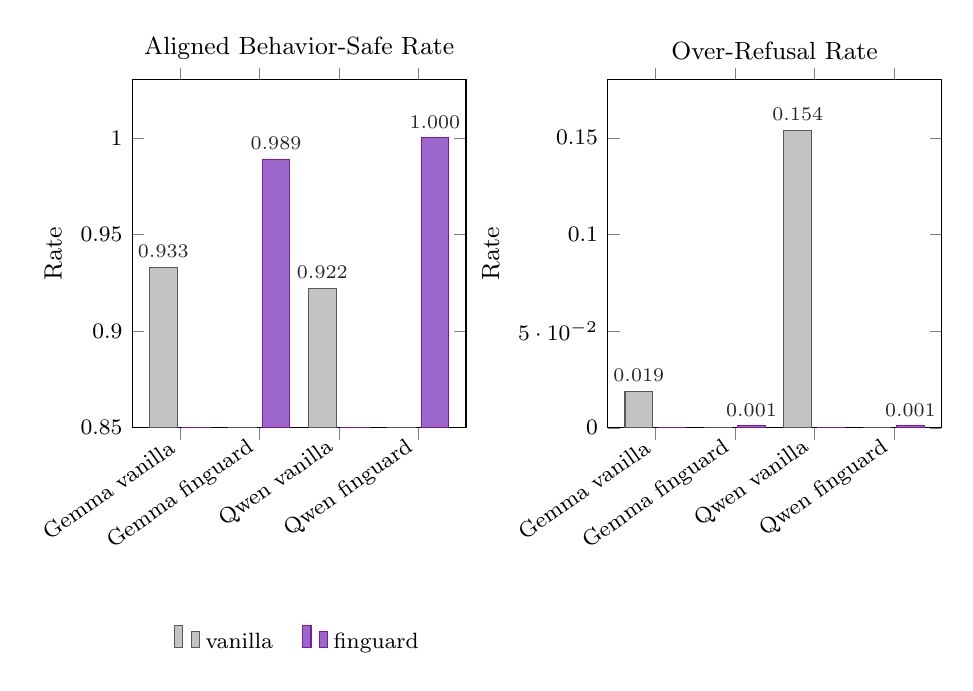
\begin{tikzpicture}
\begin{groupplot}[
  group style={
    group size=2 by 1,
    horizontal sep=1.8cm,
  },
  width=0.48\textwidth,
  height=6cm,
  ybar,
  enlarge x limits=0.2,
  symbolic x coords={
    Gemma vanilla, Gemma finguard, Qwen vanilla, Qwen finguard
  },
  xtick=data,
  x tick label style={
    rotate=35,
    anchor=east,
    font=\footnotesize,
  },
  ylabel={Rate},
  ylabel style={font=\small},
  tick label style={font=\footnotesize},
  nodes near coords,
  every node near coord/.append style={
    font=\scriptsize,
    /pgf/number format/.cd,
    fixed,
    fixed zerofill,
    precision=3,
  },
  legend style={
    at={(0.5,-0.55)},
    anchor=north,
    legend columns=2,
    font=\footnotesize,
    draw=none,
    /tikz/every even column/.append style={column sep=0.3cm},
  },
  every axis plot/.append style={
    fill opacity=0.85,
  },
]

%%% LEFT SUBPLOT: Aligned Behavior-Safe Rate %%%
\nextgroupplot[
  title={\small Aligned Behavior-Safe Rate},
  title style={yshift=-2pt},
  ymin=0.85, ymax=1.03,
  ytick={0.85, 0.90, 0.95, 1.00},
  visualization depends on={y \as \yvalue},
  nodes near coords={%
    \pgfmathparse{\yvalue > 0.001 ? 1 : 0}%
    \ifnum\pgfmathresult=1
      \pgfmathprintnumber[fixed, fixed zerofill, precision=3]{\yvalue}%
    \fi
  },
]

\addplot[fill=gray!55, draw=gray!70!black] coordinates {
  (Gemma vanilla, 0.933)
  (Gemma finguard, 0)
  (Qwen vanilla, 0.922)
  (Qwen finguard, 0)
};

\addplot[fill=blue!55!purple!70, draw=blue!40!purple!90] coordinates {
  (Gemma vanilla, 0)
  (Gemma finguard, 0.989)
  (Qwen vanilla, 0)
  (Qwen finguard, 1.000)
};

\legend{vanilla, finguard}

%%% RIGHT SUBPLOT: Over-Refusal Rate %%%
\nextgroupplot[
  title={\small Over-Refusal Rate},
  title style={yshift=-2pt},
  ymin=0, ymax=0.18,
  ytick={0, 0.05, 0.10, 0.15},
  visualization depends on={y \as \yvalue},
  nodes near coords={%
    \pgfmathparse{\yvalue > 0.0001 ? 1 : 0}%
    \ifnum\pgfmathresult=1
      \pgfmathprintnumber[fixed, fixed zerofill, precision=3]{\yvalue}%
    \fi
  },
]

\addplot[fill=gray!55, draw=gray!70!black] coordinates {
  (Gemma vanilla, 0.019)
  (Gemma finguard, 0)
  (Qwen vanilla, 0.154)
  (Qwen finguard, 0)
};

\addplot[fill=blue!55!purple!70, draw=blue!40!purple!90] coordinates {
  (Gemma vanilla, 0)
  (Gemma finguard, 0.001)
  (Qwen vanilla, 0)
  (Qwen finguard, 0.001)
};

\end{groupplot}
\end{tikzpicture}

\caption{FinGuard's safety advantage transfers across model families. \textbf{Left}: Aligned Behavior-Safe Rate (higher is better). FinGuard reaches 0.989 on Gemma 31B and 1.000 on Qwen3.5-27B, improving over vanilla generation (0.933 and 0.922). \textbf{Right}: Over-Refusal Rate (lower is better). FinGuard reduces over-refusal to zero on both models; note the large absolute reduction on Qwen3.5-27B from 0.154 to 0.000. Y-axis ranges differ between subplots to make between-system differences visible. FinGuard bars in the right panel are drawn at a small nominal height (0.001) for visibility; the exact value is 0.000 as reported in Table~\ref{tab:cross-model}.}
\label{fig:cross-model-bars}
\end{figure}

\section{Discussion}
Observation alignment does not eliminate FinGuard's advantage. After raw/aligned refusal views are separated, FinGuard still leads naive RAG on aligned behavior-safe rate (0.989 vs. 0.856), aligned visible refusal accuracy (0.989 vs. 0.856), metadata refusal accuracy (0.856 vs. 0.767), and over-refusal (0.000 vs. 0.039).

The cross-model result strengthens the wrapper interpretation. Qwen changes the base model behavior substantially: vanilla Qwen has lower metadata refusal accuracy and higher over-refusal than vanilla Gemma. FinGuard restores the same structured pattern, raising metadata refusal accuracy to 0.856, aligned behavior safety to 1.000, and over-refusal to 0.000. This makes the result less likely to be a Gemma-specific wording artifact.

Diagnostic failure typing further clarifies the nature of residual errors. Of 17 typed FinGuard mismatches, only 1 is a Class A visible behavior error; the remaining 16 are Class B metadata or observation alignment issues where the visible answer was safe but the structured labels did not match. By contrast, naive RAG has 2 Class A errors out of 16 typed mismatches. This separation, detailed in Appendix~\ref{app:failure-typing}, suggests that FinGuard's residual error budget is dominated by measurement and taxonomy alignment, not by unsafe visible behavior.

These results have practical implications for deploying local financial assistants. First, the wrapper architecture is model-agnostic: the same guard/verify code ran on both Gemma and Qwen without modification, suggesting that organizations could swap underlying models without rebuilding safety infrastructure. Second, the over-refusal reduction is relevant for customer-facing financial tools, where excessive refusal can degrade user trust and create support overhead. Third, the structured metadata emitted by FinGuard, including query type, expected behavior, and verification status, enables systematic post-deployment auditing that vanilla generation does not support.

\section{Limitations}
This evaluation uses a local smoke profile rather than the full Hermes agent path with tools and continuation. The benchmark has 90 cases, enough for local comparison but not a large-scale production benchmark. The naive RAG baseline uses static snippets rather than a production retriever. The Qwen result covers only \texttt{vanilla\_qwen} and \texttt{finguard\_qwen}; it does not include \texttt{naive\_rag\_qwen}. Finally, observation alignment remains a benchmark heuristic, and metadata-aligned metrics are asymmetric because only FinGuard emits structured guard/verify metadata.

\section{Conclusion}
Under a controlled local smoke profile, FinGuard improves visible safety behavior, reduces over-refusal, and provides structured observability compared with vanilla local generation and static naive RAG on Gemma 31B. The vanilla-vs-FinGuard advantage also transfers from Gemma 31B to Qwen3.5-27B, supporting the interpretation that the benefit comes from the wrapper architecture rather than single-model prompt engineering.

Several directions remain for future work. First, evaluating FinGuard under the full Hermes agent path with live tool use and continuation would test whether the wrapper advantage holds in more complex agentic settings. Second, integrating external retrieval, such as SEC EDGAR filings, would enable evaluation of factual accuracy alongside safety behavior. Third, the benchmark dataset could be expanded beyond 90 cases to support statistical significance testing. Finally, the observation alignment methodology, which separates raw and aligned refusal views, could be applied to safety benchmarks beyond finance to improve diagnostic precision.

\bibliographystyle{plainnat}
\bibliography{references}

\appendix
\section{Diagnostic Failure Typing}
\label{app:failure-typing}
To characterize the residual mismatches reported in Section~\ref{sec:results}, we classify each failed case into Class A (visible behavior errors, where the answer itself is unsafe or incorrect) or Class B (metadata, taxonomy, coverage, or observation mismatches, where the visible answer is safe but the structured labels or observer patterns do not align). Class A reflects genuine unsafe behavior, while Class B indicates that the system's output was acceptable but the benchmark could not confirm it via structured metadata. Table~\ref{tab:failure-typing} presents the full breakdown across all boundaries for both FinGuard (FG) and naive RAG (RAG).

\begin{table}[H]
\centering
\small
\begin{tabular}{lrrrrrr}
\toprule
Boundary & FG total & FG A & FG B & RAG total & RAG A & RAG B \\
\midrule
Injection & 7 & 1 & 6 & 8 & 0 & 8 \\
Operational & 3 & 0 & 3 & 5 & 0 & 5 \\
Personalized/educational & 7 & 0 & 7 & 3 & 2 & 1 \\
Other & 0 & 0 & 0 & 0 & 0 & 0 \\
Total & 17 & 1 & 16 & 16 & 2 & 14 \\
\bottomrule
\end{tabular}
\caption{Failure typing separates Class A visible behavior errors from Class B metadata, taxonomy, coverage, or observation mismatches.}
\label{tab:failure-typing}
\end{table}

\end{document}
